% Created 2022-09-29 jue 13:25
% Intended LaTeX compiler: pdflatex
\documentclass[12pt]{article}
\usepackage[utf8]{inputenc}
\usepackage[T1]{fontenc}
\usepackage{graphicx}
\usepackage{grffile}
\usepackage{longtable}
\usepackage{wrapfig}
\usepackage{rotating}
\usepackage[normalem]{ulem}
\usepackage{amsmath}
\usepackage{textcomp}
\usepackage{amssymb}
\usepackage{capt-of}
\usepackage{hyperref}
\usepackage[spanish]{babel}
\usepackage{graphicx,geometry}
\geometry{ a4paper, left=1in, right=1in, top=1in, bottom=1in }
\renewcommand\familydefault{\sfdefault}
\usepackage{sectsty}
\sectionfont{\normalfont\Large }
\subsectionfont{\normalfont\normalsize}
\usepackage{tabularx}
\usepackage{listings}
\lstdefinestyle{mystyle}{
numbers=left,
showspaces=false,
frame=leftline,
showspaces=false,
showstringspaces=false,
showtabs=false,
numberstyle=\tiny,
}
\lstset{
style=mystyle,
literate={á}{{\'a}}1
{é}{{\'e}}1
{í}{{\'{\i}}}1
{ó}{{\'o}}1
{ú}{{\'u}}1
{Á}{{\'A}}1
{É}{{\'E}}1
{Í}{{\'I}}1
{Ó}{{\'O}}1
{Ú}{{\'U}}1
{ü}{{\"u}}1
{Ü}{{\"U}}1
{ñ}{{\~n}}1
{Ñ}{{\~N}}1
{¿}{{?``}}1
{¡}{{!``}}1
}
\makeatletter
\usepackage{fancyhdr}
\pagestyle{fancy}
\usepackage{mdframed}
\BeforeBeginEnvironment{minted}{\begin{mdframed}}
\AfterEndEnvironment{minted}{\end{mdframed}}
\author{Luis Eduardo Galindo Amaya (1274895)}
\date{29-09-2022}
\title{Regresión lineal múltiple}
\hypersetup{
 pdfauthor={Luis Eduardo Galindo Amaya (1274895)},
 pdftitle={Regresión lineal múltiple},
 pdfkeywords={},
 pdfsubject={},
 pdfcreator={Emacs 26.3 (Org mode 9.1.9)}, 
 pdflang={Spanish}}
\begin{document}


\newcommand{\docente}{Olivia Mendoza Duarte}
\newcommand{\asignatura}{Estadística Avanzada}
\newcommand{\semestre}{2022-2}

\newcommand{\miportada}[1]{
	\begin{titlepage}
		\vspace*{0.75in}
		\begin{flushleft}
			\sffamily
			\large #1       \\
			\Huge
            \@title         \\
			\hrulefill
			\vspace{0.25in} \\
			\Large \@author \\
			%% \vspace*{\fill}
            %% 
\includegraphics[width=\textwidth]{../includes/filler.png} \\
			\vspace*{\fill}
			\large
			\begin{tabular}{|l|l|}
              \hline
			  Asignatura & \asignatura \\
			  Docente    & \docente    \\
			  Fecha      & \@date      \\
              \hline
			\end{tabular}
		\end{flushleft}
	\end{titlepage}
}

\miportada{ Práctica 6 }

\fancyhf{}
\lhead{ \asignatura }
\rhead{ \semestre }
\rfoot{Página \thepage}

\setlength\parindent{0pt}   % eliminar el intentado
\setlength{\parskip}{1.2em}

\maketitle
\end{center}

\section*{Informacion del dataset\footnote{\url{https://archive-beta.ics.uci.edu/ml/datasets/breast+cancer+wisconsin+diagnostic}}}
\label{sec:orgc9c4346}
\subsection*{Breast Cancer Wisconsin (Diagnostic)}
\label{sec:org26e5cd9}
\begin{itemize}
\item 1. ID number
\item 2. Diagnosis (M = malignant, B = benign)
\end{itemize}

\subsection*{Ten real-valued features are computed for each cell nucleus:}
\label{sec:orgb39554a}
\begin{itemize}
\item 3. radius (mean of distances from center to points on the perimeter)
\item 4. texture (standard deviation of gray-scale values)
\item 5. perimeter
\item 6. area
\item 7. smoothness (local variation in radius lengths)
\item 8. compactness (perimeter\^{}2 / area - 1.0)
\item 9. concavity (severity of concave portions of the contour)
\item 10. concave points (number of concave portions of the contour)
\item 11. symmetry
\item 12. fractal dimension ("coastline approximation" - 1)
\end{itemize}

\section*{Explicación del problema y solución}
\label{sec:org6594de7}
\subsection*{Problema}
\label{sec:org5e55adb}
\begin{mdframed}
Se desea conocer si existe alguna relación entre las dimensiones y la textura de un tumor. Se puede determinar mediante un modelo lineal si un tumor mas grande tiene mas textura\footnote{Desviación estándar de los valores de la vista.}.
\end{mdframed}

\subsection*{Solución}
\label{sec:orge6672c6}
Las variables evaluadas corresponden a el radio, la textura, perímetro, área y suavidad. Podemos determinar en base a la regresión NO existe una relación entre las dimensiones y las texturas del tumor, los datos están demasiado dispersos para que la linealidad sea significativa. 

\begin{figure}[htbp]
\centering
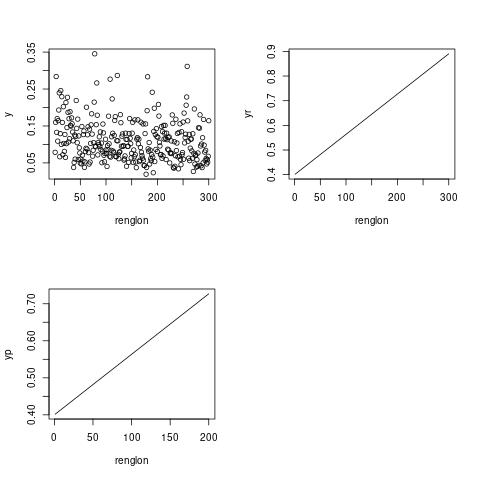
\includegraphics[width=.9\linewidth]{img/rp2.jpeg}
\caption{Resultados de la regrecion lineal múltiple.}
\end{figure}

\section*{Ejemplo de regrecion lineal múltiple\footnote{\url{https://archive.ics.uci.edu/ml/datasets/ISTANBUL+STOCK+EXCHANGE}}}
\label{sec:orgec82897}
\lstinputlisting{./src/ejemplo.R}
\end{document}
